\section{Multi-Agent Quality Audit}
\label{sec:audit}

The audit pipeline runs every generated question through nine automated
agents organised into four teams (Figure~\ref{fig:audit}). Each agent
emits a per-question signal in $\{\textsc{pass}, \textsc{warn},
\textsc{fail}\}$ and signals are calibrated against a human-reviewed
gold sheet using Cohen's $\kappa$. Agents whose human agreement falls
below threshold are downweighted to advisory-only, on the principle that
an automated judge whose verdict humans cannot reproduce should not gate
question admission. A separate human-review web application
(Appendix~\ref{app:screenshots}) collects the gold-sheet ratings from
WSET-Diploma reviewers and is itself part of the released artifact set.

\begin{figure}[t]
  \centering
  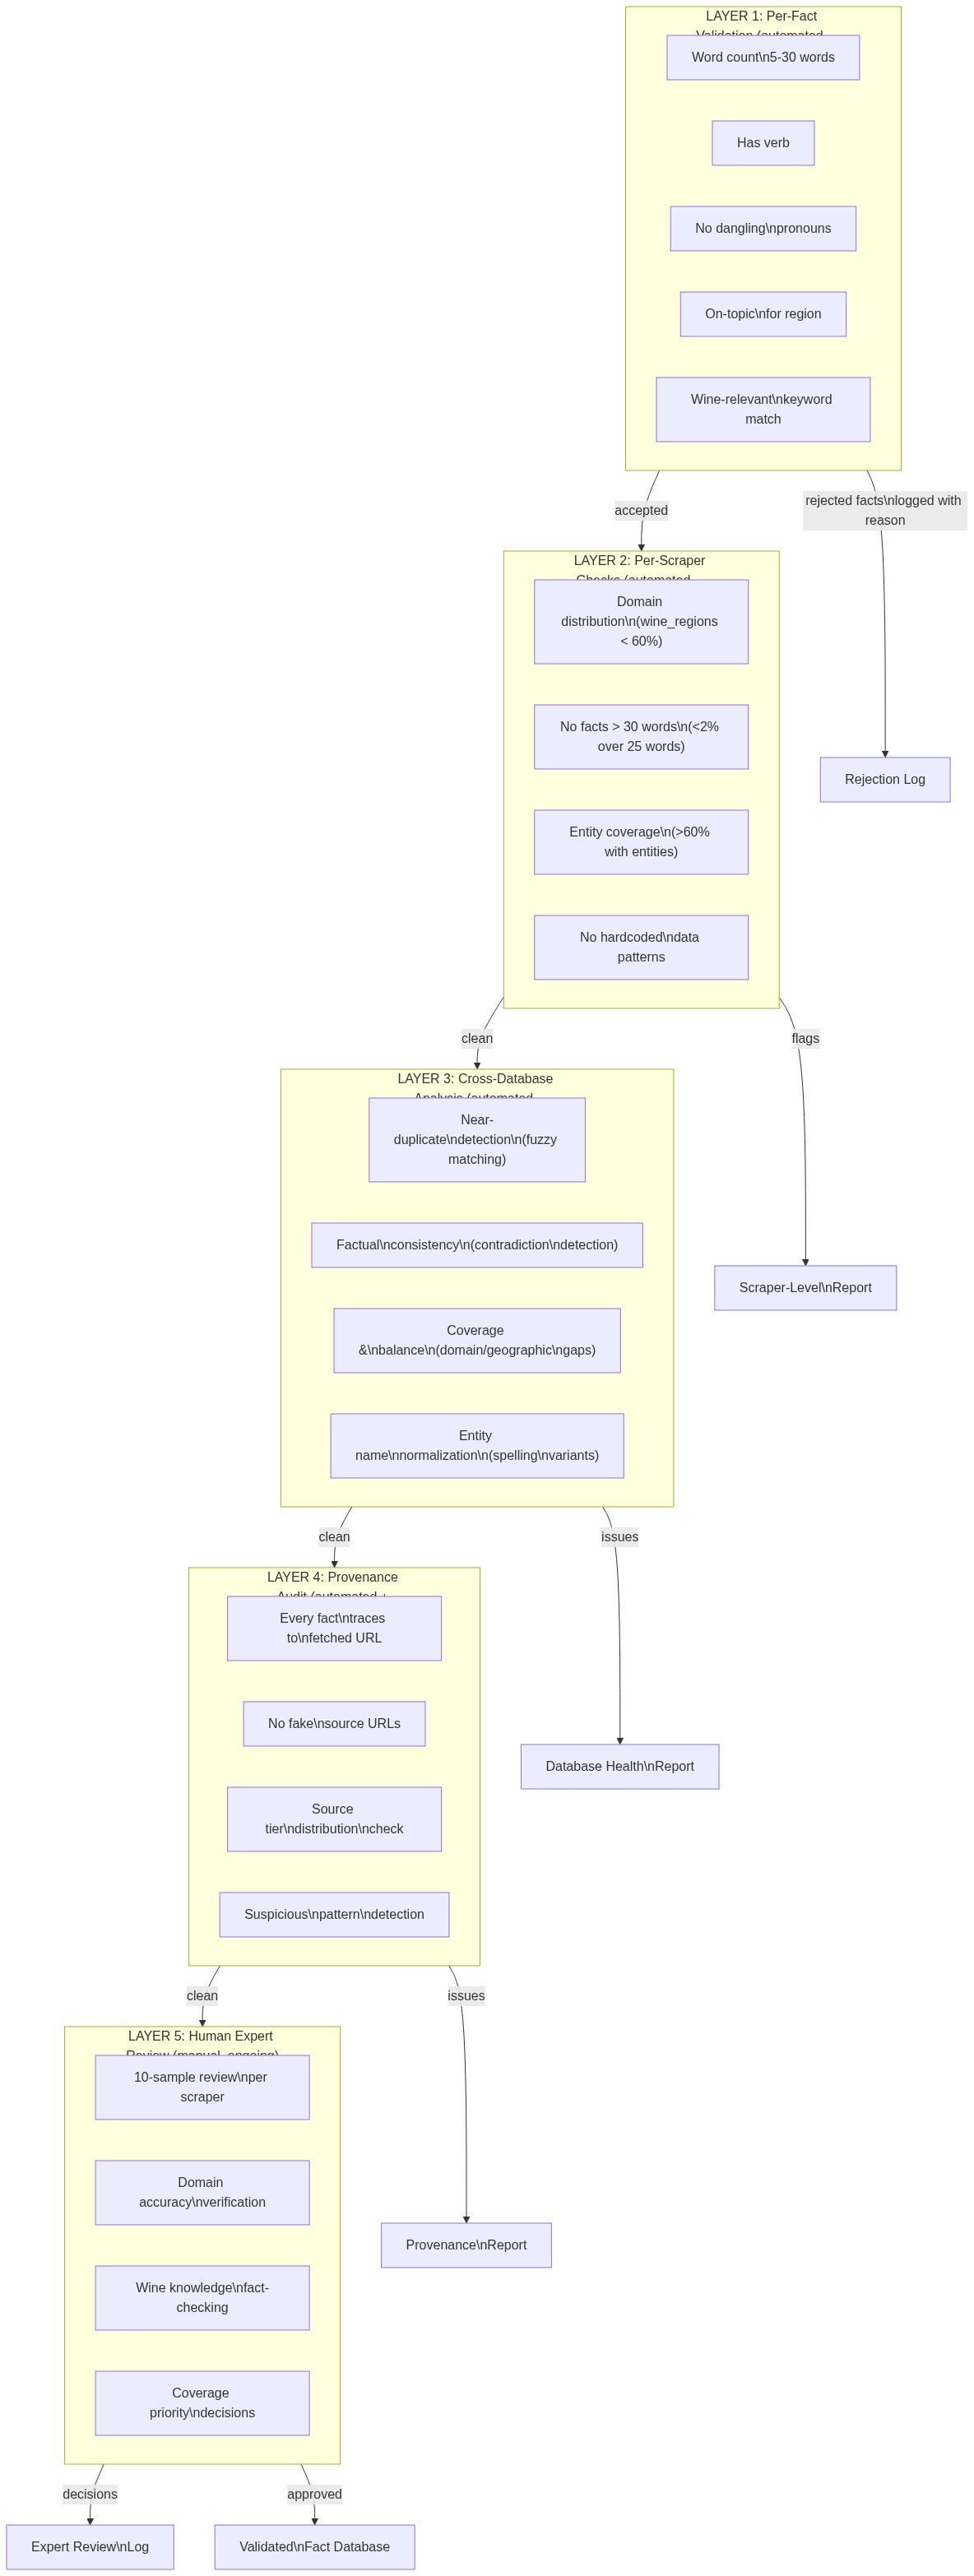
\includegraphics[width=0.92\linewidth]{figures/diagram_quality_assurance.png}
  \caption{Five-layer quality assurance stack. Per-fact and per-scraper
    checks (L1--L2) gate ingestion; cross-database consistency and
    provenance audit (L3--L4) gate corpus-level promotion; the
    multi-agent audit and human gold-sheet review (L5) gate the final
    release. Each layer feeds rejection logs back to the source.}
  \label{fig:audit}
\end{figure}

\subsection{Team architecture}
\label{sec:audit-arch}

\begin{table}[h]
  \centering
  \caption{Nine audit agents across four teams. Static agents use no
    LLM; tri-judge agents use a panel of three frontier models with
    majority voting.}
  \label{tab:agents}
  \footnotesize
  \begin{tabular}{llp{0.55\linewidth}}
    \toprule
    Team & Agent & Function \\
    \midrule
    \multirow{4}{*}{A. Static}    & A1 LexicalHygiene      & Regex sweep for vague phrasing, marketing language, meta-questions. \\
                                  & A2 BiasStats           & $\chi^2$ on correct-answer position; Mann--Whitney $U$ on correct-vs-distractor length. \\
                                  & A3 FactEcho            & Longest-common-substring ratio between question text and source fact (\textsc{fail} at LCS$\geq$0.65). \\
                                  & A4 TemplateFingerprint & POS-bigram logistic regression detector for template-induced stylistic regularities (held-out AUC 0.84). \\
    \midrule
    \multirow{2}{*}{B. Tri-judge} & B1 TriJudgeAnswer      & Claude / GPT / Gemini panel reads question + source fact and votes on the marked-correct option. \\
                                  & B2 ClosedBookSolvability & Same panel, source fact \emph{withheld}: can the question be answered from world knowledge alone? \\
    \midrule
    \multirow{2}{*}{C. Determ.}   & C2 CategoryLeak        & Wine-type distractor validation; flags red/white/sparkling category mismatches. \\
                                  & C4 DifficultyAudit     & Gemini Pro re-rates difficulty; \textsc{fail/warn} when delta $\geq$2 from assigned. \\
    \midrule
    D. Population                  & D1/D3 Skew \& SPS      & Country/sub-domain over-representation; per-generator self-vs-other accuracy. \\
                                  & B3 UbiquityRisk        & Internationally-grown grape stem $\times$ region-class answer $\Rightarrow$ ambiguity flag. \\
    \bottomrule
  \end{tabular}
\end{table}

Five additional agents (C1 DistractorDifficulty, C3 SourceSwap, B4
Ambiguity, D2 DedupCalibration, plus an escalation-only B5 verifier) are
implemented but \emph{escalation-gated}: they are invoked only when an
upstream agent flags a corpus-level concern. This deferred-execution
policy keeps routine audit cost bounded ($\sim$\$76 for the full corpus
audit reported here, 5h~22m wall) while preserving full coverage when a
defect class is suspected. The full audit code, prompts and thresholds
are released alongside the corpus
(Appendix~\ref{app:methodology}).

\subsection{Gold-sheet calibration}
\label{sec:gold}
A human gold sheet of 50 stratified questions per release is rated by a
WSET-Diploma reviewer against eight rubrics:
\texttt{answer\_correct}, \texttt{distractors\_plausible},
\texttt{not\_ambiguous}, \texttt{source\_faithful},
\texttt{needs\_source}, \texttt{no\_vague\_language},
\texttt{labels\_correct}, and \texttt{verbatim\_copy}. For each
automated agent we compute Cohen's $\kappa$ against the corresponding
human rubric on the gold sheet. \textbf{Agent signals with $\kappa<0.6$
are downweighted to advisory-only and excluded from gating decisions.}

The most consequential calibration result concerns agent
\textbf{B2~ClosedBookSolvability}: against the human reviewer, who
solved only $\approx$12\% of the gold-sheet questions without seeing the
source fact, the LLM tri-judge panel reported $\approx$83\% solvability,
yielding $\kappa\approx0.007$. We interpret this not as a defect of the
benchmark but as a property of the \emph{evaluator}: frontier LLM judges
have absorbed enough wine knowledge during pre-training to over-attribute
``world knowledge'' to questions that humans find non-trivial. We
therefore retain the 1{,}601 B2-flagged questions in the released
corpus, document the finding in the datasheet, and report a
closed-book vs.\ source-grounded contrast in
Section~\ref{sec:eval-cb} that turns the audit's blind spot into a
calibrated diagnostic of memorisation reliance.

\subsection{Release-cycle results}
\label{sec:audit-results}
The 9-agent audit on \texttt{release\_v1.1} (3{,}670 candidate questions,
run \texttt{2ba38269}) produced the verdicts in Table~\ref{tab:audit_results}.

\begin{table}[h]
  \centering
  \caption{Audit findings on \texttt{release\_v1.1} and the resulting
    drop / re-label policy.}
  \label{tab:audit_results}
  \footnotesize
  \begin{tabular}{lrl}
    \toprule
    Audit signal & Triggered FAIL & Action \\
    \midrule
    A1 LexicalHygiene (vague phrasing)               & 60   & drop \\
    A3 FactEcho (verbatim copy)                      & 63   & drop \\
    B1 TriJudgeAnswer (wrong answer key)             & 47   & drop \\
    C2 CategoryLeak (wine-category leak)             & 9    & drop \\
    B3 UbiquityRisk (grape $\times$ region ambiguity)& 183  & drop \\
    \midrule
    Distinct dropped (with overlap)                  & \textbf{341} & \\
    \midrule
    C4 DifficultyAudit (relabel from 1{,}252 LLM hits + 7 human)
                                                     & 1{,}259 & re-label \\
    B2 ClosedBookSolvability (kept w/ disclosure)     & 1{,}601 & disclose \\
    \bottomrule
  \end{tabular}
\end{table}

After drops, a follow-up post-evaluation pass (Section~\ref{sec:eval}
and Appendix~\ref{app:eval}) audited the 97 questions that all 16
evaluation configs answered incorrectly: 54 were removed as defects
(wrong ground truth, all-correct options, duplicate options), 9 were
dropped on borderline-review and the remaining 34 retained as
legitimately hard. The final released corpus is 3{,}266 questions.

The C4-driven difficulty re-label was decisive: it shifted the corpus
from 14\% L3+L4 items (the original generator-assigned distribution) to
\textbf{51\% L3+L4} (Table~\ref{tab:difficulty-shift}), bringing the
hardest-tier counts above the entry-tier counts and substantially
sharpening difficulty-stratified analyses (Section~\ref{sec:eval-rank}).

\begin{table}[h]
  \centering
  \caption{Difficulty distribution before and after C4 re-label.}
  \label{tab:difficulty-shift}
  \footnotesize
  \begin{tabular}{lrrr}
    \toprule
    & Generator-assigned & Post-relabel & $\Delta$ \\
    \midrule
    L1 (entry)        & 1{,}261 (38\%) & 694   (21\%) & $-567$ \\
    L2 (intermediate) & 1{,}559 (47\%) & 894   (27\%) & $-665$ \\
    L3 (advanced)     &   218 ( 7\%) & 678   (21\%) & $+460$ \\
    L4 (expert)       &   291 ( 9\%) & 1{,}001 (31\%) & $+710$ \\
    \bottomrule
  \end{tabular}
\end{table}

\subsection{Calibration philosophy}
We emphasise the design choice underlying these numbers. A naive
``automated audit'' interpretation would have dropped all 1{,}601
B2-flagged questions, which would have removed nearly half the corpus
and biased the remainder toward whatever idiosyncratic items the LLM
panel happened not to know. By calibrating B2 against humans and
treating it as an evaluator-side signal, we preserve dataset value while
giving downstream users a principled way to interpret leakage. The
audit's role, on this reading, is not to be the final arbiter of
quality, but to surface signals \emph{that humans validate} as
quality-relevant, and to disclose clearly the signals where humans and
LLMs disagree.
